\section{Method}
This section explains how data was collected, how the different visualizations were coded, and how the candidates were tested.

\subsection{Data Collection Pipeline}
This section will go into further detail what data was collected from Twitter and how this data was collected, prepared, and stored.

\subsubsection{Fetching the data from Twitter} \label{sec:fetchedData}
The application for collecting the tweets was written in Python 3 (\cite{10.5555/1593511}), the Twitter API was accessed using the package \emph{Tweepy} (\cite{roesslein2020tweepy}). Tweepy's connection to Twitter's Streaming API was used to collect all German tweets containing one or more of the keywords
\begin{verbatim}
    Corona, Covid-19, covidioten, distancing
\end{verbatim}. From the returned Tweet Objects\footnote{The documentation on what data a Tweet Object contains can be found here: https://developer.twitter.com/en/docs/tweets/data-dictionary/overview/tweet-object}, only a few data points were kept that seemed interesting before the data collection started. This has mainly ethical reasons (\cite{richards2014big}). The author did not want to collect excessive personal data without having a good reason to, even though this has become the norm for big data over the last decade. The following data points of a tweet object get processed further and eventually saved to a database:

\begin{itemize}
\item \textbf{The full text of the tweet.} This is mainly used for sentiment analysis and other natural language processing-tasks.
\item \textbf{The tweet's time-stamp.}
\item \textbf{The ID of the tweet.} This makes it easier to check for duplicates in the data base. 
\item \textbf{The user name of the tweet author.} As discussed above, opinion leadership is a phenomenon also on Twitter. Collecting the user names allows for later analysis, e.g., which users tweet the most.
\item \textbf{The user's self-description.} Users on Twitter can enter a short description, the so-called \emph{bio}.
\item \textbf{The user's friend count.} This shows how many other accounts the user in question is following.
\item \textbf{The user's follower count.} This shows how many other accounts follow the user in question. \footnote{The definitions for a user's friend count and follower count can be found here: https://developer.twitter.com/en/docs/accounts-and-users/follow-search-get-users/overview}
\item \textbf{The country where the tweet was sent.} Twitter also offers coordinate-based geolocations, but choosing the country instead seemed to honor the user's privacy more.
\item \textbf{Whether the account is verified or not.}
\item \textbf{The source of the tweet.} This shows if the tweet came from the Web-App, a desktop app, a mobile app, a 3rd party-application or other sources.
\item \textbf{The calculated sentiment of the tweet.} The score gets calculated during the pre-processing of the tweet. Later sections will go into more detail on how the sentiment is calculated.
\end{itemize}

%TODO: Add figure how the data was collected (it's in miro)

Twitter's \emph{Streaming API} was used as it gives the most complete data set on Twitter's free tier (\cite{bruns2014}). It pushes (or streams) tweets that match the above-mentioned criteria to a specified endpoint the moment such a tweet gets sent on Twitter. An alternative to using the streaming API is to access Twitter's archive. However, the functionality of the archive is severly limited on the free tier of the Twitter API. Using the free tier, it is only possible to collect data from the last seven days, and even then the data set is not complete. Because of this, the streaming API was used in this study.

Using the streaming API meant, however, that the application had to run 24/7: the streaming API streams the data as it comes in and doesn't save it on Twitter's network. To ensure constant availability, the python application that connects to the streaming API and processes the incoming tweets runs in a Docker Container (\cite{merkel2014docker}) on Google's App Engine (\cite{google2020}). This made it easy to set up a server-less infrastructure with high availability.

\subsubsection{Data processing during the collection}
Every time the Streaming API sent a tweet to the app collecting the data, a sentiment score for the tweet text was calculated. For this, the Natural Language Toolkit (NLTK) was used (\cite{loper2002nltk}). NLTK uses a dictionary-based approach for sentiment analysis. This means that NLTK uses a corpus that is coded with different sentiment scores (\cite{haselmayer2017sentiment}). These scores are then summed up to calculate the overall sentiment of the tweet.
Compared with machine learning-approaches, this approach high precision, but low recall (\cite{soroka2015}). This means that the polarity of a sentiment as computed by NLTK is usually correct; however, many texts that do carry a specific sentiment are not recognized and are as such marked as texts with neutral sentiments.
A machine-learning-based approach for calculating sentiments was also considered. However, the tool would have required a server which runs a Java application. This would have meant a second instance of Google AppEngine, doubling the costs. Considering that the goal of this study is to test how laymen work with the dataset, and not a scientific analysis of the discussion about the coronavirus in the German twittersphere, the dictionary-based approach was chosen to keep down the costs.

\subsubsection{Storing the pre-processed tweets}
Tweets collected via the Streaming API are bundled to batches of 100. These batches then get published as a message to a \emph{Pub/Sub Topic}. According to Google, \say{Pub/Sub is an asynchronous messaging service that decouples services that produce events from services that process events} (\cite{google2020a}). In this case, collecting the tweets gets decoupled from writing the tweets to a data base. This approach has multiple advantages. For one, the database connection does not need to be open constantly. This makes the pipeline more robust: if the database connection is closed---for whatever reason---the messages published to the pub/sub topic is saved for up to 30 days. Once the database connection is re-established, the messages get ingested and the tweets are added to the data base. It also allowed for some early experimentation with the table schema for the SQL table. Pub/Sub could be configured so that already acknowledged messages stay in the system and can be fetched again. This meant that even though the table schema was constantly reset in the first couple of days of data collection, the data was not lost and could simply be re-fetched again.

The tweets are stored in a \emph{Google BigQuery} database, a server-less data warehouse that allows fast analysis of large amounts of data (\cite{google2020b}). \emph{Google Firebase} was also considered as data storage (\cite{google2020c}). As Firebase is a NoSQL database, the database queries would have been easier to write: Instead of using SQL, standard Javascript could have been used. This would have resulted in easier queries as Javscript features, like method chaining, would have been available. Seeing that the SQL-based BigQuery is better equipped to handle large amounts of data, this solution was chosen in the end. This turned out to be a good choice considering that the final dataset was almost 1GB big and that during an average testing session the data set was queried around 5 times. However, using BigQuery meant that the queries needed to be written in SQL, a language with complicated semantics (\cite{slutz1998massive}).

BigQuery was chosen over other SQL databases, like SQLite or Postgres, because it is also a Google service like AppEngine. This meant that authentication between the script collecting the tweets and the database did not have to be implemented. BigQuery can also be directly connected to a Pub/Sub-Topic using Google DataFlow. However, as the data were additionally processed, saving the data was handled in a dedicated script. 

\subsection{Visualizing the data}
To visualize the data from the streaming API, both Python libraries like ggplot (\cite{wickham2016}) and JavaScript libraries like D3 (\cite{bostock}) and VegaLite (\cite{uwidl}) were evaluated. To make the prototype as accessible as possible, a JavaScript based library was chosen, as JavaScript is a popular web technology. A web page is more accessible to laymen than a Python-based app, as there is no need to install additional tooling. And even though Python scripts, including visualizations, can be embedded easily on the web now, choosing a web technology seemed like the right approach.

Ultimately, D3 was chosen as a visualization framework. VegaLite is an opinionated framework which chooses many defaults for the user, while D3 is unopinionated. This means that the visualizations are harder to code but more versatile.

Early prototypes of the tool used a Svelte-based web page to show the visualizations. The final tool, however, was written in Observable\footnote{https://observablehq.com}. Observable is a JavaScript based notebook that, similarly to Jupyter Notebooks, combine code, output, and explanatory text. The notebooks allowed for quick iteration of the code, while its web-based nature also satisfied the requirement of being easily accessible without the need to download and install additional software.

\subsubsection{Fetching and processing the data}
While D3 can work with raw data input and perform, e.g., filtering operations on these inputs, data operations were performed directly in the database using SQL queries. This decision was made because the final dataset was almost 1GB big. Relying on D3 for filtering and aggregating the data would have meant that every time a user opens the tool, she would have to wait for the whole dataset to finish downloading before she could use the tool itself. Using SQL queries instead meant that a lot less data had to be sent to the tool: instead of downloading the full 997MB of the data set, the query results were only about 10KB big which greatly improved performance.

%To explore the dataset of collected tweets, users can have three additional filters that they can use
Users could explore the data using different filters:
\begin{enumerate}
    \item A word-filter which allows users to search the data base for tweets including a specific word.
    \item A toggle wether to include retweets in the data set.
    \item A toggle wether to include neutral tweets in the data set, with \emph{neutral} meaning tweets with a sentiment between -0.3 and +0.3). %TODO: write in related work about this
\end{enumerate}

The toggles to include retweets and neutral tweets in the data set changed the visualizations immediately, whereas the word-filter initiated a new database query. The idea behind this was that users are likely to look for a specific topic and then want to explore how this topic is presented in the data set. One possible scenario is that users want to find out how the general public thinks of masks. They then enter the keyword \emph{mask} into the search field and can then explore this topic further. The first version of the dashboard made a new database call every time one of the toggles was clicked. This became an issue during pre-tests: the delay caused by the database call made it difficult to compare the visualizations with the different filters, e.g., to compare how the graph looks with or without retweets included.

Because of this, data fetching was rewritten before the user tests started. Every time a user filters for a new word, the tool fetches the data for the four different filter permutations: the full dataset, the dataset without retweets, the dataset without neutral tweets, and the dataset without retweets and neutral tweets. If the user then toggles additional filters, the corresponding pre-fetched dataset gets immediately visualized instead of fetching a new dataset from the database.

\subsubsection{The visualizations themselves}
The final prototype that was tested included two different visualizations:
\begin{enumerate}
    \item \textbf{A visualization of the tweet volume over time:} Users can explore how many tweets were sent per day. When filtering for a word, users can see how many of the tweets per day contained the word they searched for. They can also toggle a normalized view which shows the percentage of tweets containing the search word, rather than the absolute number.
    \item \textbf{A visualization of the sentiment over time:} Using this visualization, users can explore if and how the public perception of a topic changed over time. This visualization also offers two views. The default view shows two lines: one line shows the sentiment for the tweets containing the search word, the other line shows the sentiment for the tweets \emph{not} containing the search word. A toggle shows only the daily average of all tweets instead, regardless of the search word.
\end{enumerate}

Time series were chosen as the primary visualization type because they are one of the most common visualizations (\cite{heer2010}). Choosing a common visualization aids laymen to read and interpret the data more easily (\cite{borner2016}), whereas more complicated visualizations can be difficult to understand for those people. Because of this, the development of certain aspects of the dataset \emph{over time} was chosen as the primary type of information that the visualizations should convey.

\begin{figure}[h!tb]
    \fbox{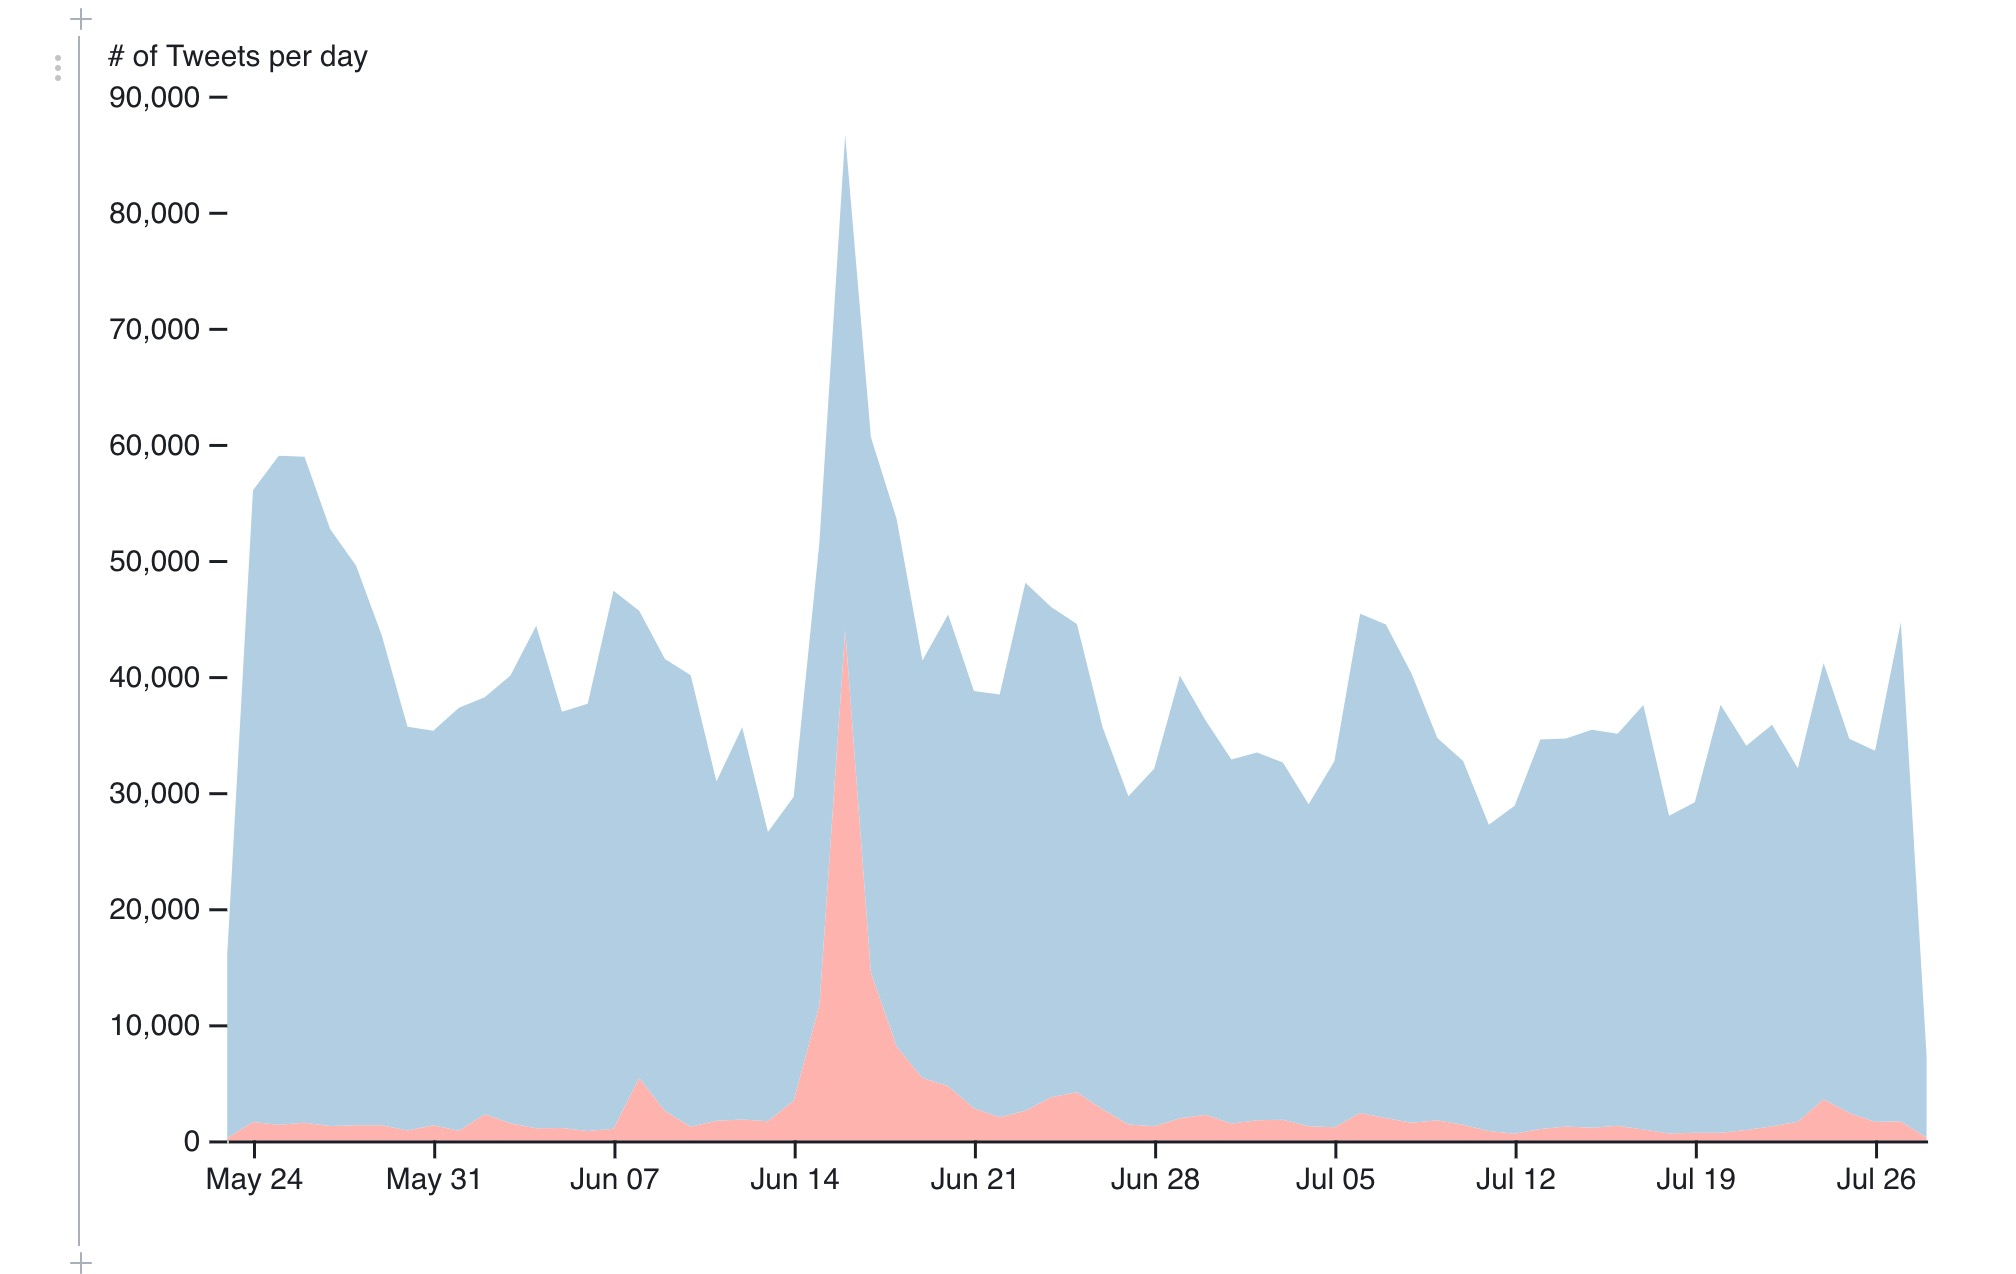
\includegraphics[width=\linewidth]{images/volume_areachart.jpg}}
    \caption{The daily tweet volume as shown in an area chart. This example shows the distribution of the word \emph{App}.}
    \label{fig:volume_areachart}
\end{figure}

To visualize the tweet volume over time, both an area chart and a bar chart were considered. Line charts and area charts are both common visualizations to show how something changed over time. Stock prices, for example, are usually shown as a line chart. An area chart is a line chart with its areas filled, which can be seen in figure \ref{fig:volume_areachart}. The filled area was used to indicate how many tweets contained the search word. However, visualizations which use line- or area charts to show development over time usually show data over a wider time range. For example, stock prices are usually shown over several years. The data set for this study spanned only around two months.

Because of this, the chart was changed to a bar chart, as seen in figure \ref{fig:volume_barchart}. Bar charts can't show information as concise as line charts or area charts. However, using a bar chart makes it easier to find and compare specific days. Using Chrome's responsive design inspector, the bar chart was pre-tested across multiple device sizes and appeared to be usable even on 11-inch displays without horizontal scrolling. The final user tests all used the bar chart visualization for the tweet volume.

\begin{figure}[h!tb]
    \fbox{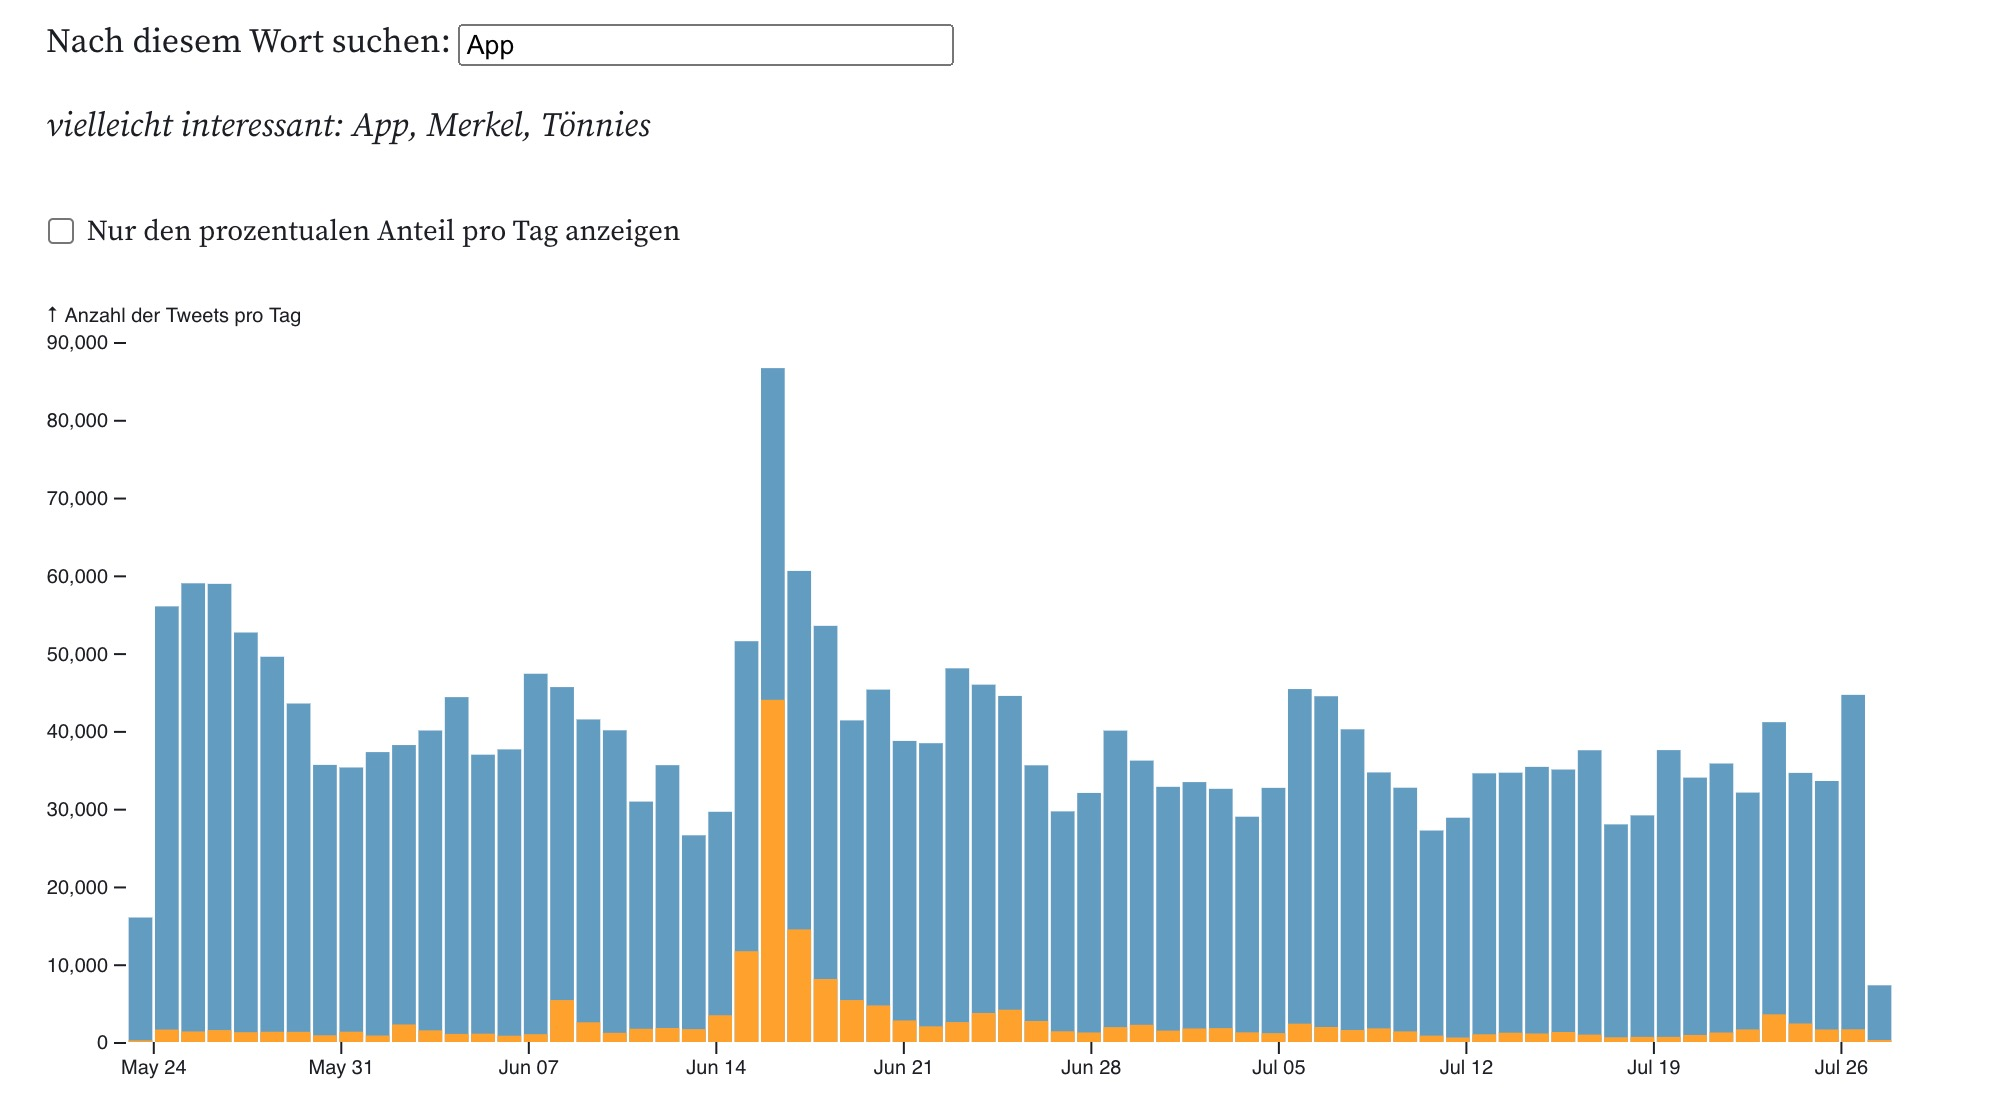
\includegraphics[width=\linewidth]{images/volume_barchart.jpg}}
    \caption{The daily tweet volume as a bar chart. This example shows the distribution of the word \emph{App}.}
    \label{fig:volume_barchart}
\end{figure}

The graph which shows the development of the sentiment over time is a line chart. This visualization was chosen because the sentiment can also show negative values, as its domain ranges from -1 to +1. 
% TODO Does this make sense? Why didn't I choose a bar chart? The line chart felt like the more natural choice here, but y tho?

\begin{figure}[h!tb]
    \fbox{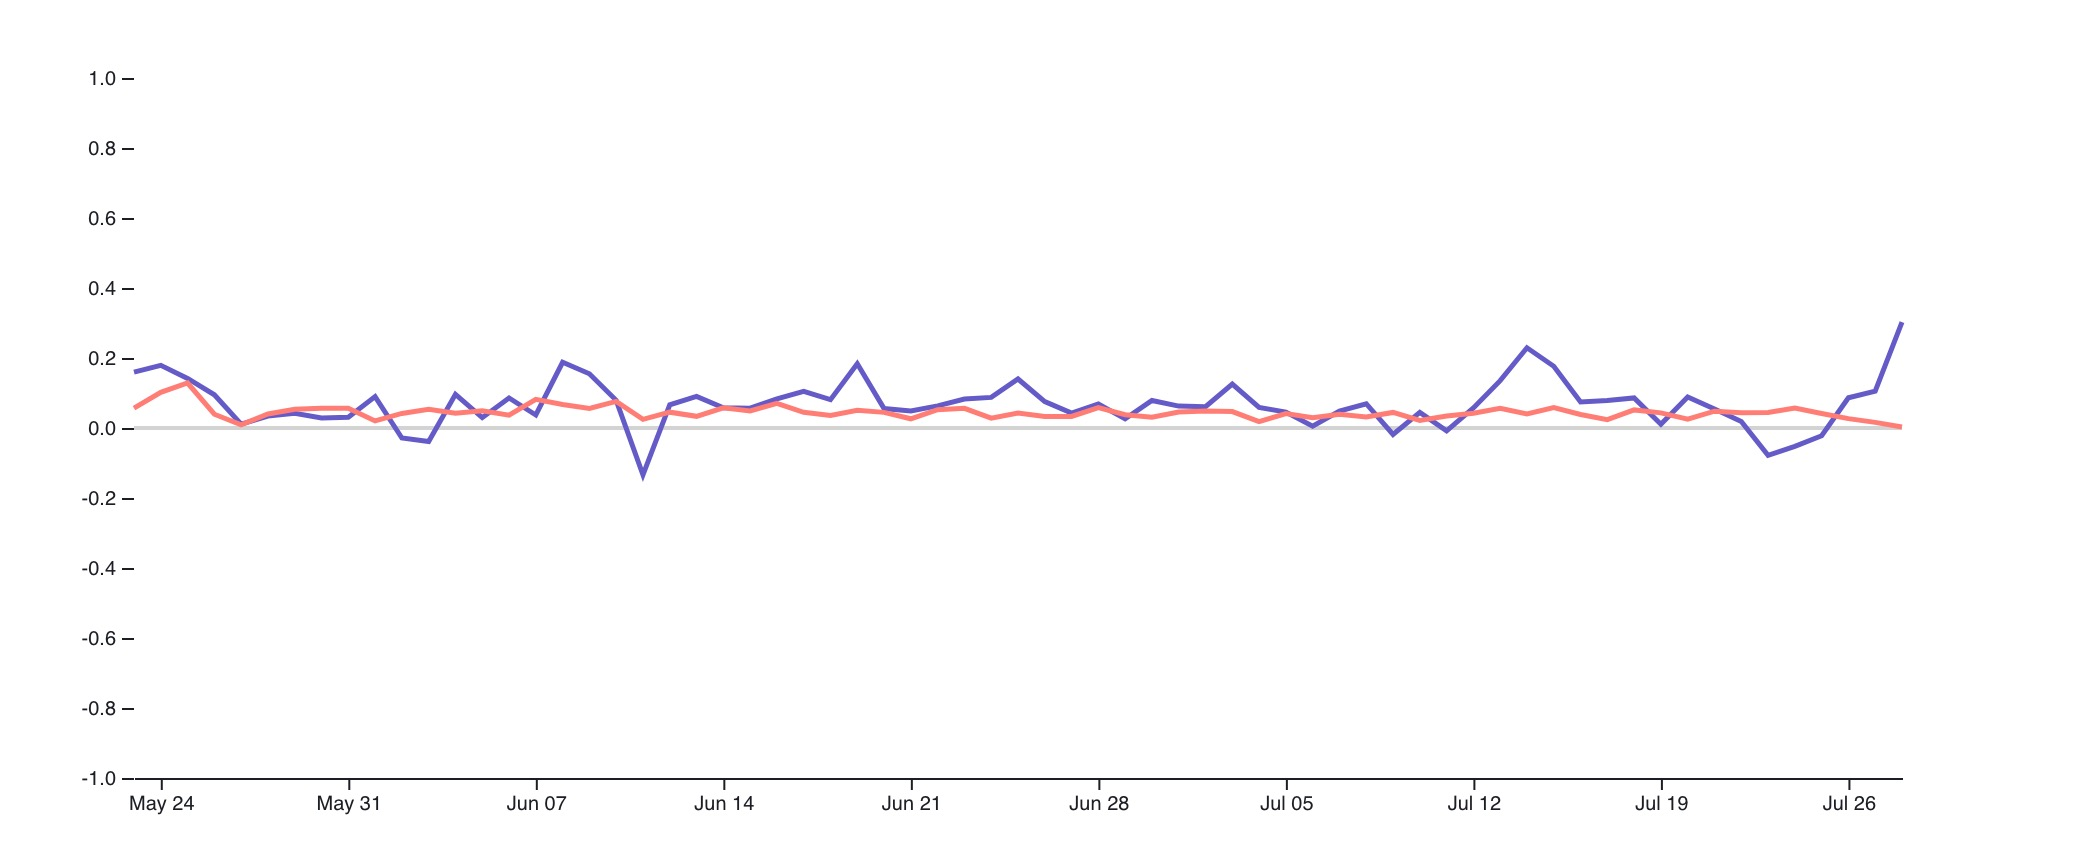
\includegraphics[width=\linewidth]{images/sentiment_linechart.jpg}}
    \caption{The average sentiment per day. The blue line shows the average sentiment of tweets containing \emph{App}, the red line shows the sentiment of tweets not containing this word.}
    \label{fig:sentiment_linechart}
\end{figure}

In this visualization, users can toggle between two view modes. The default mode shows the daily average sentiment of the tweets containing the search word as a blue line and the daily average sentiment of tweets \emph{not} containing the word as a red line. Users can also toggle to only see the average sentiment without any word-filters applied. This lets them, for example, see the influence of neutral tweets or retweets on the whole dataset.

The two visualizations share the same three aforementioned filters. This means that both visualizations share the same data set which could make it easier for participants to mentally connect them. At the same time, placing the filter possibilities at the top of the Observable notebook means that the visualizations are affected by filters that are not in their immediate neighborhood. This trade-off was tested in the user study which will be discussed later in this work.

\subsubsection{Ideas that were cut for time}
The big data pipeline and the visualization dashboard were both built using the principles of \emph{Shape Up}, a relatively new management approach for software development projects (\cite{singer2019}). The core principle of Shape Up is to have a fast time frame with a variable scope. Instead of creating a set of user stories, which then get estimates on how long they probably take, Shape Up's philosophy is to set clear boundaries, take a fixed amount of time (usually six weeks), and make the best out of the time they allowed themselves on the project. This methodology seemed like a more reasonable approach to writing a program for a master's thesis as the time frame is very strict.
Because of this, however, some ideas that were planned for the visualization dashboard were ultimately cut for time.

\begin{wrapfigure}{l}{0.3\textwidth}
    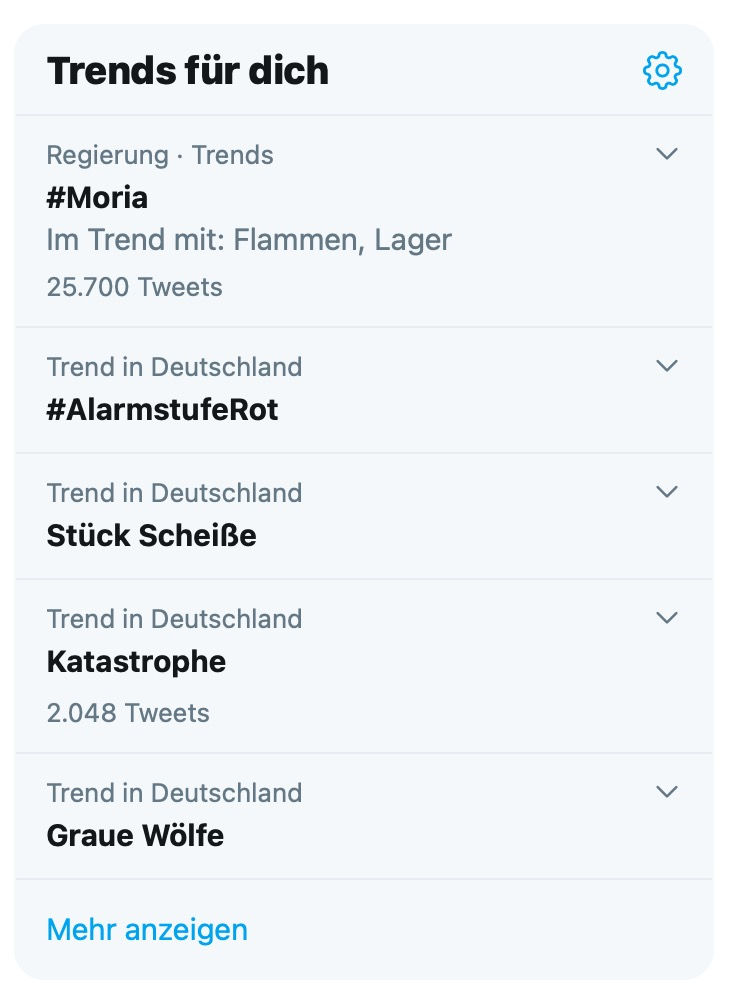
\includegraphics[width=0.28\textwidth]{images/twitter_trends.jpg}
    \caption{The trending topics on twitter. Collected on September 9th, 2020, 8.28am}
    \label{fig:twitter_trends}
\end{wrapfigure}

One feature that was not sufficiently finished when the user tests became was a sort of \emph{trend analysis} using the collected tweets. The plan was to show users trending topics for each day in the data set. Due to Twitter's limitations in their API, it was not possible to retrieve the daily trends that Twitter already collects and shows. 
To overcome this limitation, collocations were calculated for the tweet texts of each day. Collocations are \say{a lexical phenomenon} that \say{cover word pairs and phrases that are commonly used in language} (\cite[2]{mckeown2000collocations}), which means that they are word pairs that encounter together more often than by pure chance. The idea was that by calculating collocations on the tweets of a day, those word pairs could be phrases that were talked about on this day. While for some days the results seemed promising, for most of the days the calculated word pairs did not give much information. While it is possible that tweaks on the algorithm which calculated the collocations could have yielded more informative results, these tweaks could not be implemented before the user tests started.

Another feature that was planned, but not included, were tooltips in both visualizations. The tooltips were planned to include details, like the date and the specific value of the sentiment when hovering over a point on the line chart. While tooltips are generally possible in D3 for different chart types, there was no time left to properly implement them. For the bar chart, a work-around was used: Title-attributes were added to the div-containers that create the bars using the code seen in figure \ref{code:details_title}. By hovering over the bars, this title attribute is shown, which contained the date, the total number of tweets, the number of tweets containing the search word, and the percentage of tweets containing the search word. As the line chart is not built using divs per day, but rather from a single SVG element, this workaround could not be used in the chart showing the development of the sentiment over time.

\begin{figure}[h!]
    \begin{verbatim}
        svg.append("rect:title")
        .text(
        d =>
        `${formatTime(d.date)} | ${d.query_count} von ${
            d.total_count
        } Tweets (${(d.percentage * 100).toFixed(1)} %)`
    );
    \end{verbatim}
    \caption{The code that adds the date, the number of words containing the search word, the total number of tweets, and the percentage of words containing the search word to the bin of every day.}
    \label{code:details_title}
\end{figure}

As shown in chapter \ref{sec:fetchedData}, the country of origin for every tweet was collected. With this, a visualization could have shown differences in tweeting behavior between different countries. A theoretical example would be the questions if tweets about a Covid-19 vaccine that come from Russia are more positive than tweets about a vaccine that were tweeted from other countries. However, out of the 2.5 million tweets collected, only around 20,000 contained the origin country. Because of this small amount of data, this feature was not implemented.

Another data point that was collected, but ultimately not used, was the verification status of the tweets' authors. The initial plan was to offer users an option to compare tweets from verified and unverified sources. The plan was to include a toggle that breaks up the existing bar chart and line chart with another dimension \emph{is\_verified}. This would have added a lot of complexity to the visualizations for the users. Because the focus of this work is on visualizations that can be easily read and understand by laymen, this feature was eventually scrapped before the user tests.

\subsection{Testing the dashboard}
The user tests of the dashboard were testing two things: how users explore the dataset using the dashboard, and how easily they can read the two visualizations. For this, a guide for a semi-structured interview was prepared (see Appendix TODO). %TODO: Die Semi-Structured Quelle hierher packen!
The test consisted of two parts. After a brief introduction to the topic of this master thesis and a quick overview over the dataset, participants got around five minutes to explore the dashboard however they wanted. During this time, they were already asked to think aloud.

After this phase of free exploration, the participants were presented with four tasks in total with increasing difficulty. These tasks were designed to check the participants' ability to properly read the data visualizations. Again, participants were asked to think aloud while solving the tasks.
\begin{itemize}
    \item Task 1 was to find out on which day most tweets were sent. This task can be solved by finding the longest bar in the bar chart. It didn't matter which word was entered as the search word, as participants were asked to find the highest \emph{total} number of tweets, which can always be seen in blue. However, participants should toggle both neutral tweets and retweets to show up in the data set. After finding the highest bar, participants could hover over it to find the date in the tooltip.
    \item Task 2 was to find out on which day the most tweets were sent about Dr. Drosten. This search term was used to see if the participants could figure out that the search is, in fact, a filter. Only very little results were found typing in \say{Dr. Drosten}. Participants had to search for \say{Drosten} instead. This task also aimed to find out whether participants understand the difference between the day with the absolute highest number of tweets and with the relative highest number, compared to the total number of tweets that day.
    \item Task 3 was to find out how the sentiment about Dr. Drosten was when the neutral tweets were filtered out. This task tested two things: first if the quick filters were recognized as such, and if their job was clear. Then, the participants' ability and willingness to discuss ambiguous results was tested. The sentiments of tweets about Dr. Drosten changed significantly over time, with various peaks in both positive and negative sentiment as seen in figure \ref{fig:sentiment_drosten_noneutral}. Thus, there was no definite answer to the question. Participants had to read the data carefully and interpret it.
    \begin{figure}[h!tb]
        \fbox{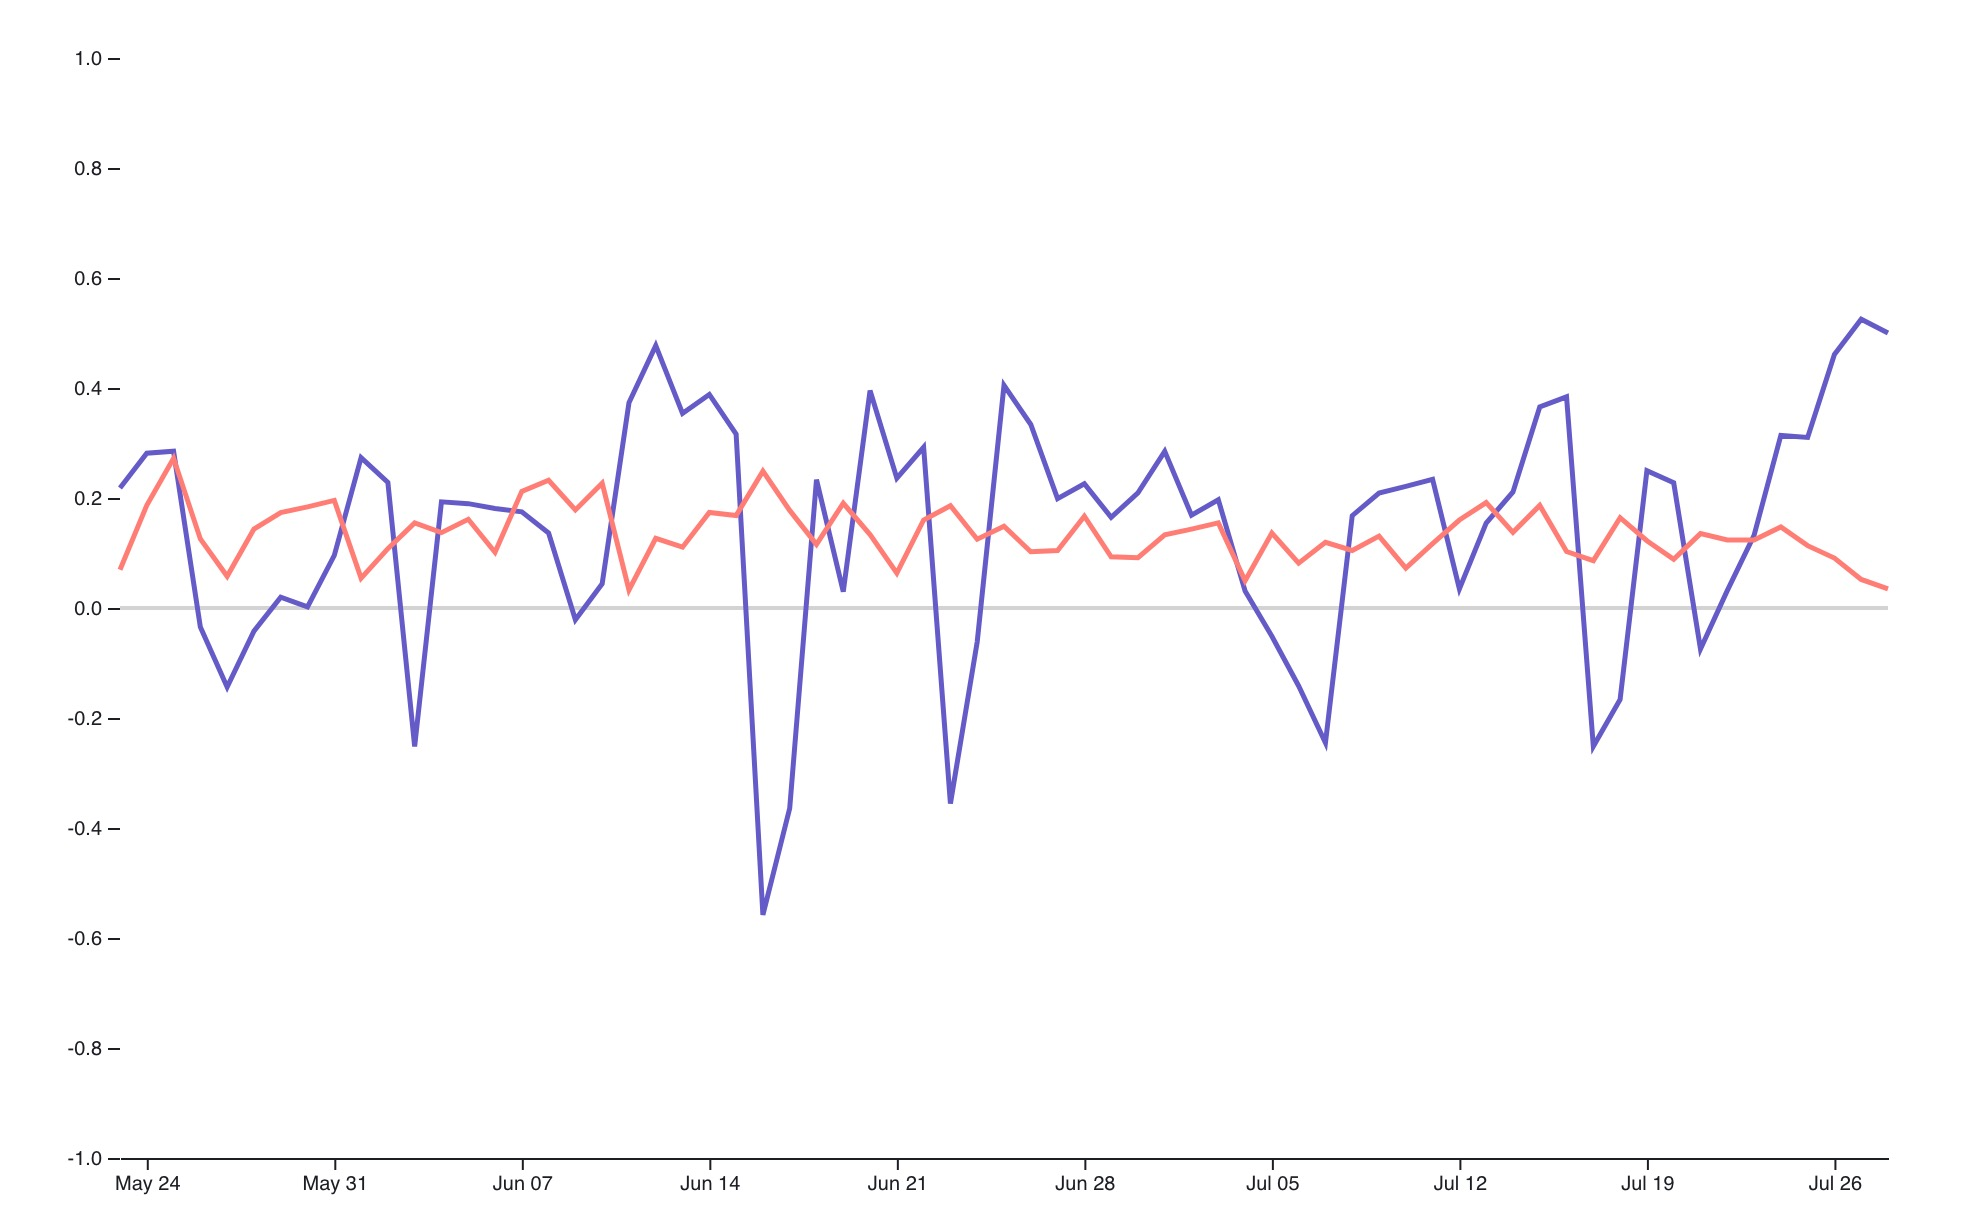
\includegraphics[width=\linewidth]{images/sentiment_drosten_noneutral.jpg}}
        \caption{The daily average sentiment of tweets containing the word \emph{Drosten}, without neutral tweets.}
        \label{fig:sentiment_drosten_noneutral}
    \end{figure}
    \item Task 4 was another task to test the participants' ability and willingness to discuss their findings. %TODO: why should they be able to discuss findings? It's important from a data literacy-perspective.
    For this final task, participants were asked to find out how retweets influence the overall sentiment of the German twitter discussion about covid-19. To solve this task, participants had to observe the influence the retweet-filter had on the sentiment graph and discuss this change. As in task 3, there is no definite right or wrong answer.
\end{itemize}

After the participants had completed the four tasks, a retrospective interview was conducted. The retrospective interview asked participants about their experience working with the tool and solving the tasks. Questions that arose during testing were also asked in the retrospective interview instead of during testing itself. Participants were also asked to report whether they had any questions in mind that they thought they should be able to answer using the dashboard.

Due to the ongoing Covid-19 pandemic, the interviews were conducted with the online video conference system Zoom\footnote{https://zoom.us}, rather than in person. Conducting the interview using Zoom had both advantages and disadvantages. On the one hand, Zoom allowed easy recording of both the audio, the screen, and the participants' webcam, which made transcribing easier. Participants could also take part in the study from their own home, rather than having to travel to a prepared test room. This made it possible to ask participants who did not live in Aachen to take part in the interviews.
On the other hand, even though Zoom does not require a lot of setup, this meant that people without access to their own internet-capable device could not participate in the study. Also, less tech-savvy people could have been hindered from participating in the study because they didn't want to or didn't know how to install Zoom and join the video conference.

The recorded zoom meetings were later transcribed to a reading version. After this, the transcriptions were coded based on Mayring's approach to qualitative content analysis (\cite{mayring2010qualitative}). For this, a deductive approach was used. Categories were derived from the material and sorted into two primary categories: \say{Motivationsfaktoren} (\emph{motivational factors}) and \say{Hemmfaktoren} (\emph{hindering factors}), based on whether the finding motivated the participants to use the tool or hindered their exploration. The code book, including anchor examples, will be discussed in the results section. 
